\documentclass[chapterprefix=false]{report}

\setlength{\oddsidemargin}{0 in}
\setlength{\evensidemargin}{0 in}
\setlength{\topmargin}{0 in}
\setlength{\textwidth}{5.7 in}
\setlength{\textheight}{8.0 in}
\setlength{\headsep}{0.75 in}
\setlength{\parindent}{0.3 in}
\setlength{\parskip}{0.1 in}

\usepackage{titlesec}

\titleformat{\chapter}{\huge}{\thechapter.}{20pt}{\huge}

\usepackage{epsf}
\usepackage{pseudocode}
\usepackage{ amssymb }
\usepackage{mathtools}
\usepackage{amsmath}
\usepackage{textcomp}
\usepackage{tikz}
\usepackage{csquotes}
\usepackage{graphicx}
\usepackage[parfill]{parskip}
\usetikzlibrary{arrows}
\tikzset{
    vertex/.style={circle,draw,minimum size=1.5em},
    edge/.style={->,> = latex'}
}



\DeclarePairedDelimiter\ceil{\lceil}{\rceil}
\DeclarePairedDelimiter\floor{\lfloor}{\rfloor}

% \usepackage{times}
% \usepackage{mathptm}

\def\O{\mathop{\smash{O}}\nolimits}
\def\o{\mathop{\smash{o}}\nolimits}
\newcommand{\e}{{\rm e}}
\newcommand{\R}{{\bf R}}
\newcommand{\Z}{{\bf Z}}
\newcommand{\h}{1.2}

\DeclareMathOperator*{\argmin}{arg\,min}
\DeclareMathOperator*{\argmax}{arg\,max}
 
\begin{document}
 
\tableofcontents{}
 
\chapter{Introduction}
 
\section{In-game Sports Analytics}

$\newline$
``The win probability graphic/discussion on ESPN is literally taking a sword and sticking it through the chest of any fun left in baseball''
\\[5pt]
\centerline{{ --- Kenny Ducey (@KennyDucey) April 2, 2017}}

$\newline$
``ESPN showing win probability is extremely good. Next up, run expectancy!''
\\[5pt]
\centerline{{\rm --- Neil Weinberg (@NeilWeinberg44) April 4, 2017}}

``Thank the Lord we have the ESPN Win Probability stat to tell us the team that's ahead has a good chance to win.''
\\[5pt]
\centerline{{\rm --- Christian Schneider (@Schneider\_CM) April 17, 2017}}

In recent years, win probability has become increasingly prevalent in sports broadcasting. Brian Burke, an NFL commentator, has posted live win-probability graphs of NFL playoff games on his website for the past few years. Earlier this year, ESPN began to post win probabilities atop the score box in televised Major League Baseball games. Despite mixed reactions from fans, as shown above, these developments represent a transition in sports broadcasting's modern narrative. 

..Make an argument for the value of in-match forecasting, despite angry reactions..

At it’s simplest, a win probability from any score line communicates how much one team or player is favored to win. This metric demonstrates an individual model’s most informed guess at how likely a player is to win the match. With the recent proliferation of online betting, in-match win probability dictates an entire market of its own. While tennis has yet to broadcast win probabilities, Betfair reportedly traded over "" million in volume over the 2015 Wimbledon Final. Furthermore, around 80$\%$ of such betting occurs while matches are in progress. Clearly, in-match win probability is of great concern to all participants in this betting market. 

%Drawing upon past research and exploring new methods, this paper searches for the most effective approach to in-match forecasting.

\section{History of Tennis Forecasting}
Plenty of research on tennis match prediction exists over the past twenty years. In (are points in tennis iid?), Klaassen and Magnus test the assumption that points in a tennis match are independent and identically distributed. Under this assumption, they construct a hierarchical Markov model in conjunction with tennis’ scoring system. From this model, they offer an analytical equation for match-win probability from any score, given each individual player’s probability of winning a point on serve (forecasting).  Barnett and Clarke then offer a method of estimating each player’s serve probability from historical data (combining player outcomes). Years later, Bevc proposed updating each player’s serve probability with a beta distribution between each point and computing the corresponding win probability with the above model (predicting the outcome). Recently, Kovalchik assessed performance of 11 different pre-match prediction models on all tour-level ATP matches in 2014.

Over the past several years, Jeff Sackmann (offer footnote to website) has released the largest publicly available tennis dataset via github. This collection contains match summaries of every ATP and WTA match in the Open Era, point-by-point summaries of nearly 100,000 matches—both tour-level and satellite--and a crowd-sourced match-charting project spanning 2800 matches, where volunteers record each shot’s type and direction in every point. While 538 and Kovalchik use Jeff Sackmann’s match data to refine their own elo system for pre-match prediction, none of the aforementioned papers have used his point-by-point dataset.

As these papers have spanned several decades, the datasets referenced among them are not consistent. ", : both test in-play models on around 500 matches from Wimbledon in 1991-94. Barnett focuses almost exclusively on a marathon match between Andy Roddick and " El Aynoui from the 2002 Australian Open. However, Jeff Sackmann has recently released the largest publicly available tennis dataset via github. This collection contains match summaries of every ATP and WTA match in the Open Era, point-by-point summaries of nearly 100,000 matches—both tour-level and satellite--and a crowd-sourced match-charting project spanning 2800 matches, where volunteers record each shot’s type and direction in every point. While 538 and Kovalchik use Jeff Sackmann’s match data to refine their own elo system for pre-match prediction, no papers on in-match prediction have used his point-by-point dataset. With over 10,000 ATP and WTA tour-level matches from 2010-2017, I compare existing approaches side-by-side and explore new methods to in-match prediction.  Just as Kovalchik does with pre-match prediction models, I attempt to find the GOAT (greatest of all-time) of in-match prediction models.

This paper combines elo ratings, a wealth of data, and current technology to provide a similar survey of which in-match prediction methods perform the best. I build upon past research by testing variations of previous state-of-the-art methods, and applying several new concepts to these datasets, from successful probability models in football and baseball, to state exploration via hidden Markov Models.

 

 
\chapter{Datasets}
 
\section{Match Datasets}
 
we get from Sackmann

\section{Point-by-Point Datasets}

\chapter{Scoring}
Tennis' scoring system consists of three levels: sets, games, and points. Consider a tennis match between two entities, $p_i$ and $p_j$. We can represent any score as $(s_i,s_j),(g_i,g_j),({x}_i,{x}_j)$ where $i$ is serving and $s_k,g_k,x_k$ represent player $k$'s score in sets, games, and points, respectively. The players alternate serve each game and continue until someone clinches the match by winning two sets (best-of-three) or three sets (best-of-five) $\footnote{The best-of-five format is typically reserved for men's grand slam and Davis Cup events}$.

The majority of in-play tennis models utilize a hierarchical Markov Model, which embodies the levels in tennis' scoring system. Barnett formally defines a representation for scores in tennis (Barnett Clarke 2002). With $p_i$ and $p_j$ winning points on serve with probabilities $f_{ij},f_{ji}$, each in-match scoreline $(s_i,s_j),(g_i,g_j),({x}_i,{x}_j)$ progresses to one of its two neighbors $(s_i,s_j),(g_i,g_j),({x}_i+1,{x}_j)$ and $(s_i,s_j),(g_i,g_j),({x}_i,{x}_j+1)$ with transition probabilities dependent on the current server. Assuming all points in a match are $iid$, we can then use the above model to recursively determine win probability:

\begin{center}
$P_m(s_i,s_j,g_i,g_j,{x}_i,{x}_j)$ = probability that $p_i$ wins the match when serving from this scoreline

$P_m(s_i,s_j,g_i,g_j,{x}_i,{x}_j) = f_{ij}*P_m(s_i,s_j,g_i,g_j,{x}_i+1,{x}_j) + (1-f_{ij}) P_m(s_i,s_j,g_i,g_j,{x}_i,{x}_j+1)$
\end{center}
In the following sections, we specify boundary values to each level of our hierarchical model. 

%With these specifications, we can analytically compute win probability at any point in the match.


\section{Modeling games}

Within a game, either $p_i$ or $p_j$ serves every point. Every game starts at (0,0) and to win a game, a player must win four or more points by a margin of at least two $\footnote{While tennis officially  refers to a game's first three points as 15,30,40 we will call them 1,2,3 for simplicity's sake}$. Consequently, all games with valid scores $(x_i,x_j)$ where $x_i+x_j \textgreater 6; |x_i-x_j| \leq 1$ are reduced to (3,3), (3,2), or (2,3). Furthermore, the win probability at (3,3) can be calculated directly. From (3,3), the server wins the next two points with probability $f_{ij}^2$, the returner wins the next two points with probability $(1-f_{ij})^2$, or both players split the two points and return to (3,3) with probability $2f_{ij}(1-f_{ij})$. Relating the game's remainder to a geometric series, we find $P_g(3,3) = \frac{f_{ij}^2}{f_{ij}^2+(1-f_{ij})^2}$.

Possible sequences of point scores in a game:

a - player $i$ wins the following point

b - player $j$ wins the following point

\begin{tikzpicture} [scale=1]
\tikzset{VertexStyle/.style = {shape = circle,inner sep=0x}}
\node[vertex] (1) at (0,0) {$0,0$};
\node[vertex] (2) at (2,.8) {$1,0$};
\node[vertex] (3) at (2,-.8) {$0,1$};
\node[vertex] (4) at (4,0) {$1,1$};
\node[vertex] (7) at (4,1.6) {$2,0$};
\node[vertex] (8) at (4,-1.6) {$0,2$};
\node[vertex] (5) at (6,.8) {$2,1$};
\node[vertex] (6) at (6,-.8) {$1,2$};
\node[vertex] (9) at (6,2.4) {$3,0$};
\node[vertex] (10) at (6,-2.4) {$0,3$};
\node[vertex] (11) at (8,1.6) {$3,1$};
\node[vertex] (12) at (8,-1.6) {$1,3$};
\node[vertex] (13) at (8,0) {$2,2$};

\node[vertex] (14) at (12,3.2) {$G_1$};
\node[vertex] (15) at (12,-3.2) {$G_1^{c}$};
\node[vertex] (16) at (10,.8) {$3,2$};
\node[vertex] (17) at (10,-.8) {$2,3$};
\node[vertex] (18) at (12,0) {$3,3$};

\draw[edge] (1) -- (2) node[midway, above] {$a$};
\draw[edge] (1) -- (3) node[midway, above] {$b$};
\draw[edge] (2) -- (4) node[midway, above] {$b$};
\draw[edge] (3) -- (4) node[midway, above] {$a$};
\draw[edge] (2) -- (7) node[midway, above] {$a$};
\draw[edge] (3) -- (8) node[midway, above] {$b$};
\draw[edge] (4) -- (5) node[midway, above] {$a$};
\draw[edge] (4) -- (6) node[midway, above] {$b$};
\draw[edge] (7) -- (9) node[midway, above] {$a$};
\draw[edge] (7) -- (5) node[midway, above] {$b$};
\draw[edge] (8) -- (6) node[midway, above] {$a$};
\draw[edge] (8) -- (10) node[midway, above] {$b$};
\draw[edge] (9) -- (11) node[midway, above] {$b$};
\draw[edge] (10) -- (12) node[midway, above] {$a$};
\draw[edge] (5) -- (11) node[midway, above] {$a$};
\draw[edge] (6) -- (12) node[midway, above] {$b$};
\draw[edge] (5) -- (13) node[midway, above] {$b$};
\draw[edge] (6) -- (13) node[midway, above] {$a$};
\draw[edge] (13) -- (16) node[midway, above] {$a$};
\draw[edge] (13) -- (17) node[midway, above] {$b$};
\draw[edge] (11) -- (16) node[midway, above] {$b$};
\draw[edge] (12) -- (17) node[midway, above] {$a$};
\draw[edge] (16) -- (18) node[midway, above] {$b$};
\draw[edge] (17) -- (18) node[midway, above] {$a$};
\draw[edge] (9) -- (14) node[midway, above] {$a$};
\draw[edge] (11) -- (14) node[midway, above] {$a$};
\draw[edge] (16) -- (14) node[midway, above] {$a$};
\draw[edge] (10) -- (15) node[midway, above] {$b$};
\draw[edge] (12) -- (15) node[midway, above] {$b$};
\draw[edge] (17) -- (15) node[midway, above] {$b$};
\draw[->, xshift=11.3cm, yshift=1cm] (18) to [bend right=50] (16) node[ sloped,midway,above] {$a$};
\draw[->, xshift=11.3cm, yshift=-1cm] (18) to [bend left=50] (17) node[ sloped,midway,above] {$b$};

\end{tikzpicture}

Boundary values:

\begin{equation}
    P_g(x_i,x_j) 
    \begin{cases}
      1, & \text{if}\ x_1=4,x_2 \leq 2 \\
      0, & \text{if}\ x_2=4,x_1 \leq 2 \\
      \cfrac{f_{ij}^2}{f_{ij}^2+(1-f_{ij})^2}, & \text{if}\ x_1=x_2=3 \\
      f_{ij}*P_g(s_i,s_j,g_i,g_j,{x}_i+1,{x}_j) + (1-f_{ij}) P_g(s_i,s_j,g_i,g_j,{x}_i,{x}_j+1), & \text{otherwise}\ \\
      
    \end{cases}
  \end{equation}

With the above specifications, we can efficiently compute player $i$'s win probability from any score $P_g(x_i,x_j)$.

\section{Modeling Sets}

Within a set, $p_i$ or $p_j$ alternate serve every game. Every set starts at (0,0). To win a set, a player must win six or more games by a margin of at least two. If the set score $(6,6)$ is reached, a special tiebreaker game is played to determine the outcome of the match.

Possible sequences of point scores in a game:

$a$ - player 1 wins the following game

$b$ - player 2 wins the following game

$a'$ - player 1 wins the tiebreaker game

$b'$ - player 2 wins the tiebreaker game

\begin{tikzpicture} [scale=.7]
\tikzset{VertexStyle/.style = {shape = circle,inner sep=0x}}
\node[vertex] (1) at (0,0) {$0,0$};
\node[vertex] (2) at (2,\h) {$1,0$};
\node[vertex] (3) at (2,-\h) {$0,1$};
\node[vertex] (4) at (4,2*\h) {$2,0$};
\node[vertex] (5) at (4,0) {$1,1$};
\node[vertex] (6) at (4,-2*\h) {$0,2$};
\node[vertex] (7) at (6,3*\h) {$3,0$};
\node[vertex] (8) at (6,\h) {$2,1$};
\node[vertex] (9) at (6,-\h) {$1,2$};
\node[vertex] (10) at (6,-3*\h) {$0,3$};
\node[vertex] (11) at (8,4*\h) {$4,0$};
\node[vertex] (12) at (8,2*\h) {$3,1$};
\node[vertex] (13) at (8,0) {$2,2$};
\node[vertex] (14) at (8,-2*\h) {$1,3$};
\node[vertex] (15) at (8,-4*\h) {$0,4$};
\node[vertex] (16) at (10,5*\h) {$5,0$};
\node[vertex] (17) at (10,3*\h) {$4,1$};
\node[vertex] (18) at (10,\h) {$3,2$};
\node[vertex] (19) at (10,-\h) {$2,3$};
\node[vertex] (20) at (10,-3*\h) {$1,4$};
\node[vertex] (21) at (10,-5*\h) {$0,5$};
\node[vertex] (22) at (18,6*\h) {$S_1$};
\node[vertex] (23) at (12,4*\h) {$5,1$};
\node[vertex] (24) at (12,2*\h) {$4,2$};
\node[vertex] (25) at (12,0) {$3,3$};
\node[vertex] (26) at (12,-2*\h) {$2,4$};
\node[vertex] (27) at (12,-4*\h) {$1,5$};
\node[vertex] (28) at (18,-6*\h) {$S_1^c$};
\node[vertex] (29) at (14,3*\h) {$5,2$};
\node[vertex] (30) at (14,\h) {$4,3$};
\node[vertex] (31) at (14,-\h) {$3,4$};
\node[vertex] (32) at (14,-3*\h) {$2,5$};
\node[vertex] (33) at (16,2*\h) {$5,3$};
\node[vertex] (34) at (16,0) {$4,4$};
\node[vertex] (35) at (16,-2*\h) {$3,5$};
\node[vertex] (36) at (18,\h) {$5,4$};
\node[vertex] (37) at (18,-\h) {$4,5$};
\node[vertex] (38) at (20,0) {$5,5$};
\node[vertex] (39) at (22,\h) {$6,5$};
\node[vertex] (40) at (22,-\h) {$5,6$};
\node[vertex] (41) at (24,0) {$6,6$};



\draw[edge] (1) -- (2) node[midway, above] {$a$};
\draw[edge] (1) -- (3) node[midway, above] {$b$};
\draw[edge] (2) -- (4) node[midway, above] {$b$};
\draw[edge] (2) -- (5) node[midway, above] {$a$};
\draw[edge] (3) -- (5) node[midway, above] {$a$};
\draw[edge] (3) -- (6) node[midway, above] {$b$};
\draw[edge] (4) -- (7) node[midway, above] {$a$};
\draw[edge] (4) -- (8) node[midway, above] {$b$};
\draw[edge] (5) -- (8) node[midway, above] {$a$};
\draw[edge] (5) -- (9) node[midway, above] {$b$};
\draw[edge] (6) -- (9) node[midway, above] {$a$};
\draw[edge] (6) -- (10) node[midway, above] {$b$};
\draw[edge] (7) -- (11) node[midway, above] {$a$};
\draw[edge] (7) -- (12) node[midway, above] {$b$};
\draw[edge] (8) -- (12) node[midway, above] {$a$};
\draw[edge] (8) -- (13) node[midway, above] {$b$};
\draw[edge] (9) -- (13) node[midway, above] {$a$};
\draw[edge] (9) -- (14) node[midway, above] {$b$};
\draw[edge] (10) -- (14) node[midway, above] {$a$};
\draw[edge] (10) -- (15) node[midway, above] {$b$};
\draw[edge] (11) -- (16) node[midway, above] {$a$};
\draw[edge] (11) -- (17) node[midway, above] {$b$};
\draw[edge] (12) -- (17) node[midway, above] {$a$};
\draw[edge] (12) -- (18) node[midway, above] {$b$};
\draw[edge] (13) -- (18) node[midway, above] {$a$};
\draw[edge] (13) -- (19) node[midway, above] {$b$};
\draw[edge] (14) -- (19) node[midway, above] {$a$};
\draw[edge] (14) -- (20) node[midway, above] {$b$};
\draw[edge] (15) -- (20) node[midway, above] {$a$};
\draw[edge] (15) -- (21) node[midway, above] {$b$};
\draw[edge] (16) -- (22) node[midway, above] {$a$};
\draw[edge] (16) -- (23) node[midway, above] {$b$};
\draw[edge] (17) -- (23) node[midway, above] {$a$};
\draw[edge] (17) -- (24) node[midway, above] {$b$};
\draw[edge] (18) -- (24) node[midway, above] {$a$};
\draw[edge] (18) -- (25) node[midway, above] {$b$};
\draw[edge] (19) -- (25) node[midway, above] {$a$};
\draw[edge] (19) -- (26) node[midway, above] {$b$};
\draw[edge] (20) -- (26) node[midway, above] {$a$};
\draw[edge] (20) -- (27) node[midway, above] {$b$};
\draw[edge] (21) -- (27) node[midway, above] {$a$};
\draw[edge] (21) -- (28) node[midway, above] {$b$};
\draw[edge] (23) -- (22) node[midway, above] {$a$};
\draw[edge] (23) -- (29) node[midway, above] {$b$};
\draw[edge] (24) -- (29) node[midway, above] {$a$};
\draw[edge] (24) -- (30) node[midway, above] {$b$};
\draw[edge] (25) -- (30) node[midway, above] {$a$};
\draw[edge] (25) -- (31) node[midway, above] {$b$};
\draw[edge] (26) -- (31) node[midway, above] {$a$};
\draw[edge] (26) -- (32) node[midway, above] {$b$};
\draw[edge] (27) -- (32) node[midway, above] {$a$};
\draw[edge] (27) -- (28) node[midway, above] {$b$};
\draw[edge] (29) -- (22) node[midway, above] {$a$};
\draw[edge] (29) -- (33) node[midway, above] {$b$};
\draw[edge] (30) -- (33) node[midway, above] {$a$};
\draw[edge] (30) -- (34) node[midway, above] {$b$};
\draw[edge] (31) -- (34) node[midway, above] {$a$};
\draw[edge] (31) -- (35) node[midway, above] {$b$};
\draw[edge] (32) -- (35) node[midway, above] {$a$};
\draw[edge] (32) -- (28) node[midway, above] {$b$};
\draw[edge] (33) -- (22) node[midway, above] {$a$};
\draw[edge] (33) -- (36) node[midway, above] {$b$};
\draw[edge] (34) -- (36) node[midway, above] {$a$};
\draw[edge] (34) -- (37) node[midway, above] {$b$};
\draw[edge] (35) -- (37) node[midway, above] {$a$};
\draw[edge] (35) -- (28) node[midway, above] {$b$};
\draw[edge] (36) -- (22) node[midway, left] {$a$};
\draw[edge] (36) -- (38) node[midway, above] {$b$};
\draw[edge] (37) -- (38) node[midway, above] {$a$};
\draw[edge] (37) -- (28) node[midway, right] {$b$};
\draw[edge] (38) -- (39) node[midway, above] {$a$};
\draw[edge] (38) -- (40) node[midway, above] {$b$};
\draw[edge] (39) -- (22) node[midway, above] {$a$};
\draw[edge] (39) -- (41) node[midway, above] {$b$};
\draw[edge] (40) -- (41) node[midway, above] {$a$};
\draw[edge] (40) -- (28) node[midway, above] {$b$};

\draw[->, xshift=20cm,yshift=6.35cm] (41) to [bend right=30] (22) node[sloped,midway,above,scale=1.4] {$a'$};
\draw[->, xshift=20cm,yshift=-6.35cm] (41) to [bend left=30] (28) node[sloped,midway,above,scale=1.4] {$b'$};


\end{tikzpicture}

Boundary values:
\begin{equation}
    P_s(g_1,g_2) 
    \begin{cases}
      1, & \text{if}\ g_1 \geq 6,g_1-g_2 \geq 2 \\
      0, & \text{if}\ g_2 \geq 6,g_2-g_1 \geq 2 \\
      P_{tb}(s_1,s_2), & \text{if}\ g_1=g_2=6 \\
      P_g(0,0)(1-P_s(g_2,g_1+1))+(1-P_g(0,0))(1-P_s(g_2+1,g_1)), & \text{otherwise}\ \\
    \end{cases}
  \end{equation}

See appendix for the tiebreak game's corresponding diagram**


\section{Modeling a best-of-three match}


a - player 1 wins the following set

b - player 2 wins the following set

\begin{tikzpicture} [scale=1]
\node[vertex] (1) at (0,0) {$0,0$};
\node[vertex] (2) at (2,1) {$1,0$};
\node[vertex] (3) at (2,-1) {$0,1$};
\node[vertex] (4) at (4,0) {$1,1$};
\node[vertex] (5) at (6,1) {$W_1$};
\node[vertex] (6) at (6,-1) {$W_1^{c}$};

\draw[edge] (1) -- (2) node[midway, above] {$a$};
\draw[edge] (1) -- (3) node[midway, above] {$b$};
\draw[edge] (2) -- (4) node[midway, above] {$b$};
\draw[edge] (3) -- (4) node[midway, above] {$a$};
\draw[edge] (2) -- (5) node[midway, above] {$a$};
\draw[edge] (3) -- (6) node[midway, above] {$b$};
\draw[edge] (4) -- (5) node[midway, above] {$a$};
\draw[edge] (4) -- (6) node[midway, above] {$b$};

\end{tikzpicture}

Boundary values:
\begin{equation}
    P_m(s_1,s_2) 
    \begin{cases}
      1, & \text{if}\ g_1 \geq 2 \\
      0, & \text{if}\ g_2 \geq 2 \\
      P_s(0,0)(P_m(s_1+1,s_2))+(1-P_s(0,0))(P_m(s_1,s_2+1)), & \text{otherwise}\ \\
    \end{cases}
  \end{equation}

Combining the above equations, we can recursively calculate win probability with player $i$ serving from $(s_i,s_j,g_i,g_j,{x}_i,{x}_j)$ as:

$P_m(s_i,s_j,g_i,g_j,{x}_i,{x}_j) = f_{ij}*P_m(s_i,s_j,g_i,g_j,{x}_i+1,{x}_j) + (1-f_{ij}) P_m(s_i,s_j,g_i,g_j,{x}_i,{x}_j+1) \newline 
= P_g(x_i,x_j)*(1-P_m(s_j,s_i,g_j,g_i+1,0,0)) + (1-P_g(x_i,x_j))*(1-P_m(s_j,s_i,g_j+1,g_i,0,0)) \newline
= 
P_g(x_i,x_j)*(1-(P_s(g_j,g_i+1)*P_m(s_j+1,s_i)+(1-P_s(g_j,g_i+1))*P_m(s_j,s_i+1)) + (1-P_g(x_i,x_j))*(1-(P_s(g_j+1,g_i)*P_m(s_j+1,s_i)+(1-P_s(g_j+1,g_i))*P_m(s_j,s_i+1)) = ...$


\chapter{Pre-game Match Prediction}

\section{Overview}
Before play has started, an in-match prediction model cannot draw on information from the match itself. Then, before a match between players $i$ and $j$ commences, it makes sense that this model should use the most well-informed pre-match forecast $\hat{\pi}_{ij}(t)$ as a starting point for predictions. Therefore, we first explore pre-match models as a starting point for in-match prediction.

Earlier this year, Kovalchik released a survey of eleven different pre-match prediction models, assessing them side-by-side in accuracy, log-loss, calibration, and discrimination. 538's elo-based model and the Bookmaker Consensus Model performed the best. Elo-based prediction incorporates player $i$ and $j$'s entire match histories, while the BCM model incorporates all information encoded in the betting market. However, the paper leaves out a point-based method  devised by Klaassen and Magnus that derives serving probabilities from historical player data (combining player outcomes).

\section{Elo Ratings}
Elo was originally developed as a head-to-head rating system for chess players (1978). Recently, 538's elo variant has gained prominence in the media. For match $t$ between $p_i$ and $p_j$ with elo ratings $E_i(t)$ and $E_j(t)$, $p_i$ is forecasted to win with probability:

\begin{center}
$\hat{\pi}_{ij}(t) = (1 + 10^\frac{E_j(t)-E_i(t)}{400})^{-1}$
\end{center}

$p_i$'s rating for the following match $t+1$ is then updated accordingly:

\begin{center}
$E_i(t+1) = E_i(t) + K_{it}*(W_i(t)-\hat{\pi}_{ij}(t))$
\end{center}

$W_i(t)$ is an indicator for whether $p_i$ won the given match, while $K_{it}$ is the learning rate for $p_i$ at time $t$. According to 538's analysts, elo ratings perform optimally when allowing $K_{it}$ to  decay slowly over time (How We're Predicting). With $m_i(t)$ representing the $p_i$'s career matches played at time $t$ we update our learning rate:

\begin{center}
$K_{it} = \frac{250}{(5+m(t))^{.4}} $
\end{center}

This variant updates a player's elo most quickly when we have no information about a player and makes smaller changes as $m_i(t)$ accumulates. To apply this elo rating method to our dataset, we initalize each player's elo rating at $E_i(0)=1500$ and match history $m_i(0)=0$. Then, we iterate through all tour-level matches from 1968-2017 $\footnote{tennis' Open Era began in 1968, when professionals were allowed to enter grand slam tournaments. Before then, only amateurs played these events}$ in chronological order, storing $E_i(t),E_j(t)$ for each match and updating each player's elo accordingly.

\section{ATP/WTA Rank}
While Klaassen and Magnus incorporated ATP rank into their prediction model (forecasting 2003), Kovalchik and 538 concur that elo outperforms ranking-based methods. On ATP match data from 2010-present, we found:

Table with elo vs ATP/WTA rank

Considering their superiority to ATP rank in 21st-century matches, models in this paper use elo ratings to represent a player's ability.

\section{Point-based Model}
The hierarchical Markov Model offers an analytical solution to win probability $\hat{\pi}_{ij}(t)$ between players $p_i$ and $p_j$, given serving probabilities $f_{ij}$,$f_{ji}$. Klaassen and Magnus outline a way to estimate each player's serving probability from historical serve and return data. 

\begin{center}
$f_{ij} = f_t + (f_i-f_{av})-(g_j-g_{av})$
%\newline

$f_{ji} = f_t + (f_j-f_{av})-(g_i-g_{av})$
\end{center}

Each player's serve percentage is a function of their own serving ability and their opponent's returning ability. $f_t$ denotes the average serve percentage for the match's given tournament, while $f_i,f_j$ and $g_i,g_j$ represent player $i$ and $j$'s percentage of points won on serve and return, respectively. $f_{av},g_{av}$ are tour-level averages in serve and return percentage. Since all points are won by either server or returner, $f_{av} =1-g_{av}$.

As per Klaassen and Magnus' implementation, we use the previous year's tournament serving statistics to calculate $f_t$ for a given tournament and year, where $(w,y)$ represents the set of all matches played at tournament $w$ in year $y$.

\begin{center}
$f_t(w,y) = \frac{\sum_{k \in (w,y-1)}{\text{\# of points won on serve in match k}}}{\sum_{k \in (w,y-1)}\text{\# of points played in match k}}$
\end{center}

Klaassen and Magnus only apply this method to a single match (Roddick vs. El Aynaoui Australian Open 2003). Furthermore, their ability to calculate serve and return percentages is limited by aggregate statistics supplied by atpworldtour.com. That is, they can only use year-to-date serve and return statistics to calculate $f_i,g_i,f_j,g_j$. Since the statistics do not list corresponding sample sizes, they must assume that each best-of-three match lasts 165 points, which adds another layer of uncertainty to estimating players' abilities.

Implementing this method with year-to-date statistics proves troublesome because $f_i,g_i$ decrease significantly in uncertainty as player $i$ accumulates matches throughout the year. Due to availability of data, match forecasts in September will then be far more reliable than ones made in January. However, with our tour-level match dataset, we can keep a year-long tally of serve/return statistics for each player at any point in time. Where $(p_i,y,m)$ represents the set of $p_i$'s matches in year $y$, month $m$, we obtain the following statistics $\footnote{for the current month m, we only collect month-to-date matches} $:

\begin{center}
$f_i(y,m) = \frac{\sum_{t=1}^{12}\sum_{k \in (i,y-1,m+t)}{\text{\# of points won on serve by i in match k}}}{\sum_{t=1}^{12}\sum_{k \in (i,y-1,m+t)}\text{\# of points played on serve by i in match k}}$
%\newline
$g_i(y,m) = \frac{\sum_{t=1}^{12}\sum_{k \in (i,y-1,m+t)}{\text{\# of points won on return by i in match k}}}{\sum_{t=1}^{12}\sum_{k \in (i,y-1,m+t)}\text{\# of points played on return by i in match k}}$
\end{center}

Keeping consistent with this format, we also calculate $f_{av},g_{av}$ where $(y,m)$ represents the set of tour-level matches played in year $y$, month $m$:

\begin{center}
$f_{av}(y,m) = \frac{\sum_{t=1}^{12}\sum_{k \in (y-1,m+t)}{\text{\# of points won on serve in match k}}}{\sum_{t=1}^{12}\sum_{k \in (y-1,m+t)}\text{\# of points played in match k}} = 1 - g_{av}(y,m)$
\end{center}

Now, variance of $f_i,g_i$ no longer depends on time of year. Since the number of points won on serve are recorded in each match, we also know the player's number of serve/return points played. Below, we combine player statistics over the past 12 months to produce $f_{ij},f_{ji}$ for Kevin Anderson and Fernando Verdasco's 3rd round match at the 2013 Australian Open.

\begin{center}
\begin{tabular}{ |c|c|c|c|c|c|c| } 
 \hline
 player name & $\#$ s points won & $\#$ s points
&$f_i$ & $\#$ r points won & $\#$ r points & $g_i$ \\ 
 \hline
 Kevin Anderson & 3292 & 4842 & .6799 & 1726 & 4962 & .3478\\ 
 \hline
 Fernando Verdasco & 2572 & 3981 & .6461 & 1560 & 4111 & .3795\\ 
 \hline
\end{tabular}
\end{center}

From 2012 Australian Open statistics, $f_t=.6153$. From tour-level data spanning 2010-2017, $f_{av} = 0.6468; g_{av} = 1-f_{av} =.3532$ Using the above serve/return statistics from 02/12-01/13, we can calculate:

\begin{center}
$f_{ij} = f_t + (f_i-f_{av})-(g_j-g_{av}) = .6153 + (.6799-.6468) - (.3795-.3532) = .6221$
%\newline
$f_{ji} = f_t + (f_j-f_{av})-(g_i-g_{av}) = .6153 + (.6461-.6468) - (.3478-.3532) = .6199$
\end{center}

With the above serving percentages, Kevin Anderson is favored to win the best-of-five match with probability $M_p(0,0,0,0,0,0) = .5139$


\section{James-Stein Estimator}
Decades ago, Efron and Morris described a method to estimate groups of sample means (Efron Morris 1977). The James-Stein estimator shrinks sample means toward the overall mean, in proportion to its estimator's variance. Regardless of the value of $\theta$, this method has proven superior to the MLE method (reporting the sample mean for each group), an admissible estimator.

To estimate serve/return parameters for players who do not regularly play tour-level events, $f_i,g_i$ must be calculated from limited sample sizes. Consequently, match probabilities based off these estimates may be skewed by noise. The James-Stein estimators offer a more reasonable estimate of serve and return ability for players with limited match history. 

%Players who do not regularly play tour-level events must yield serve and return estimates $f_i,g_i$ based on limited sample sizes. 

To shrink serving percentages, we compute the variance of all recorded $f_i$ statistics $\footnote{each ${f_i}$ is computed from the previous twelve months of player data}$ in our match data set $D_m$.

$\hat{\tau}^2 = \sum_{f_i \in D_m} (f_i-f_{av})^2$

Then, each estimator $f_i$ is based off $n_i$ service points. With each estimator $f_i$ representing $f_i/n_i$ points won on serve, we can compute estimator $f_i$'s variance and a corresponding normalization coefficient:

\begin{center}
$\hat{\sigma_i}^2 = \frac{f_i(1-f_i)}{n_i}$

$B_i = \frac{\hat{\sigma_i}^2}{\hat{\tau}^2+\hat{\sigma_i}^2}$
\end{center}

Finally, the James-Stein estimator takes the form: 

\begin{center}
$JS(f_i) = f_i + B_i(f_{av}-f_i)$
\end{center}

We repeat the same process with $g_i$ to obtain James-Stein estimators for return statistics.

To see how shrinkage makes our model robust to small sample sizes, consider the following example. When Daniel Elahi (COL) and Ivo Karlovic (CRO) faced off at ATP Bogota 2015, Elahi held only one tour-level match in his year-long stats. From a previous one-sided victory, his serve percentage, $f_i=51/64=.7969$, was abnormally high compared to the year-long tour-level average of $f_{av}=.6423$. 


\begin{center}
\begin{tabular}{ |c|c|c|c|c|c|c|c| } 
 \hline
 player name & $\#$ s points won & $\#$ s points
 & $f_i$ &$\#$ r points won & $\#$ r points & $g_i$ & elo rating \\ 
 \hline
 Daniel Elahi & 51 & 64 & .7969 & 22 & 67 & .3284 & 1516.9178 
 \\
 \hline
 Ivo Karlovic & 3516 & 4654 & .7555 & 1409 & 4903 & .2874 & 1876.9545 \\ 
 \hline
\end{tabular}
\end{center}

\begin{center}
$f_{ij} = f_t + (f_i-f_{av})-(g_j-g_{av}) = .6676 + (.7969-.6423) - (.2874-.3577) = .8925$

$f_{ji} = f_t + (f_j-f_{av})-(g_i-g_{av}) = .6676 + (.7555-.6423) - (.3284-.3577) = .8101$
\end{center}

Following Klaassen and Magnus' method of combining player outcomes, we estimate that Elahi has an $89.3\%$ chance of winning points on serve. This is extremely high, and eclipses Karlovic's $81.01\%$ serve projection. This is strange, given that Karlovic is one of the most effective servers in the history of the game. From the serving stats, our hierarchical Markov Model computes Elahi's win probability as $M_p(0,0,0,0,0,0) = .8095$. This forecast seems unreasonably confident of Elahi's victory, despite only having collected his player statistics for one match. Karlovic's 360-point elo advantage, which calculates Elahi's win probability as $\hat{\pi}_{ij}(t) = (1+10^\frac{1876.9545 - 1516.9178}{400})^{-1} = .1459$, leads us to further questions the validity of this approach when using limited historical data. Thus, we turn to the James-Stein estimator to normalize Elahi's serving and return probabilities.

\begin{center}
$JS(f_i) = f_i + B_i(f_{av}-f_i) = .7969 + .7117(.6423-.7969) = .6869$

$JS(g_i) = g_i + B_i(g_{av}-g_i) = .3284 + .7624(.3577-.3284) = .3507$

$JS(f_j) = f_j + B_j(f_{av}-f_j) = .7555 + .0328(.6423-.7555) = .7518$

$JS(g_j) = g_i + B_j(g_{av}-g_j) = .2874 + .0420(.3577-.2874) = .2904$

$JS(f_{ij}) = f_t + (JS(f_i)-f_{av})-(JS(g_j)-g_{av}) = .6676 + (.6869-.6423) - (.2904-.3577) = .7795$

$JS(f_{ji}) = f_t + (JS(f_j)-f_{av})-(JS(g_i)-g_{av}) = .6676 + (.7518-.6423) - (.3507-.3577) = .7841$

\end{center}

given $JS(f_i),JS(f_j): M_p(0,0,0,0,0,0) = .4806$

Above, we can see that the James-Stein estimator shrinks Elahi's stats far more than Karlovic's, since Karlovic has played many tour-level matches in the past year. By shrinking the serve/return statistics, our model lower's Elahi's inflated serve percentage and becomes less vulnerable to small sample sizes.

Since overly confident forecasts can hurt model performance with respect to cross entropy, the James-Stein estimator allows a safer way to estimate outcomes of matches with lesser-known players. Later on, we will use the James-Stein estimator to normalize not only year-long serve/return statistics, but also surface-specific and opponent-adjusted statistics.

%A loss by Machado in this circumstance would increase the overall log-loss of our dataset by $\approx 10^7$


%While this does not hurt our model's accuracy, such high-probability forecasts are harmful to a model's log-loss in the case of tail events. When a relatively unknown player squares off against a tour-level regular, there is a tail probability that an upset occurs.

%If Machado were to have lost against Tursunov, then our cross entropy would increase by $\approx 22$, a huge penalty for a single data point. Given Tursunov's elo advantage, this is not a situation to which we want to expose models forecasting. In the end, the James-Stein estimator offers robustness to serve/return probabilities derived from infrequently charted players. We will hold onto these estimates for use in future models.

\section{Opponent-Adjusted Serve/Return Statistics}

To do: explain equation for adjusting $f_{av},g_{av}$ in the Klaassen-Magnus Equation.

\section{Results}
The following results were obtained from testing methods on 2014 ATP best-of-three matches, excluding Davis Cup. There were 2409 matches in this dataset. Five-fold validation was used for the logit() method.

\begin{center}
\begin{tabular}{ |c|c|c|c|c| } 
 \hline
 method & accuracy & log loss
 &  &  \\ 
 \hline
  elo & 69.2 & .587
 &  &  \\ 
 \hline
 surface elo & 68.6 & .590
 &  &  \\ 
 \hline
 elo 538 & 69.3 & .595
 &  &  \\ 
 \hline
 surface elo 538 & 69.7 & .595
 &  &  \\ 
 \hline
 logit (elo 538, surface elo 538) & 69.4 & .578
 &  &  \\ 
 \hline
 
\end{tabular}
\end{center}

By combining elo and surface elo, we achieve a log loss of .58. Aside from the Bookmaker Consensus Model, which draws information directly from the betting market, no other model is documented as doing this well. Kovalchik's non-surface elo method achieved a log loss of .60 (2017). While Sipko claimed to have achieved 4.3$\%$ ROI off the betting market with a neural net, the best of his machine learning models achieves a log loss of .61 (2014). As Sipko surveyed logistic regression, the common-opponent model, and an artificial neural net, we are confident in moving forward with elo to discern a starting place for in-match prediction models.

The following methods were trained on 2010-2013 match data and tested on 2014 ATP match data.

\begin{center}
\begin{tabular}{ |c|c|c|c|c| } 
 \hline
 input & train accuracy & test accuracy
& train log loss & test log loss \\ 
 \hline
  elo & & 69.2 & & .587
   \\ 
 \hline
 surface elo & & 68.6 & & .590
  \\ 
 \hline
 elo 538 & & 69.3 & & .595 \\ 
 \hline
 surface elo 538 & & 69.7 & & .595 \\ 
 \hline
 elo/surface elo &  &  &  & \\ 
 \hline
 KM &  &  &  & \\ 
 \hline
 KM James-Stein &  &  &  & \\ 
 \hline
  KM Surface &  &  &  & \\ 
 \hline
 KM Surface James-Stein &  &  &  & \\ 
 \hline
 KM adjusted &  &  &  & \\ 
 \hline
 KM adjusted James-Stein &  &  &  & \\ 
 \hline
\end{tabular}
\end{center}

It is important to note that Klaassen and Magnus' method of combining player statistics involves no optimization with respect to a training dataset. Of the above methods, only a logistic regression with elo and surface elo actually learns its model parameters with respect to a training dataset. 



\chapter{In-game Match Prediction}
Having surveyed all relevant pre-match prediction models, we proceed to in-match prediction. Since the most commonly used in-match prediction models utilize the hierarchical Markov Model structure, all previously computed serving percentages may also be tested on an in-match probability model. To start, we will test several machine-learning methods as a baseline.

The following methods will be tested primarily on tour-level matches for which we have point-by-point data. The matches span 2010-2017, accounting for nearly half of all tour-level matches within this time. Point-by-point records in Sackmann's dataset take the form of the following string:

Mikhail Youzhny vs. Evgeny Donskoy Australian Open 2013

P=``SSRSS;RRRR;SRSSS;SRRSRSSS;SRSSRS;RSRSSS;SRSRSS;RSRSRSSS;SSSS.SSSRRRSS;

RSSSS;SSRSS;SSSRS;SSSS;RRRSSSSRRSSRRSRSSS;SRSRSS;SSSRS;RSRSSRSS;SSSS;SRSSS;

RSRSSRRSSS;R/SR/SS/RR/RS/SR.RSRRR;...''

$S$ denotes a point won by the server and $R$ a point won by the returner. Individual games are separated by ``$;$'' sets by ``$.$'' and service changes in tiebreaks by ``$/$''. By iterating through the string, one can construct $n$ data points $\{P_0,P_1,...,P_{n-1}\}$ from a match with $n$ total points, with $P_i$ representing the subset of the match after $i$ points have been played.

$P_0 = ``"$

$P_1 = ``S"$

$P_2 = ``SS"$

$P_3 = ``SSR"$

...

With $M = \{M_1,M_2,...M_k\}$ complete match-strings in our point-by-point data set, the size of our enumerated data set then becomes $\sum_{i=1}^k |M_i|$. This comes out to 1231122 points for ATP matches and "" for WTA matches.

\section{Logistic Regression}

As a baseline, we first consider a logistic regression model. 

From any scoreline  ($s_i,s_j,g_i,g_j,{x}_i,{x}_j$), we can simply feed these parameters into our model. Logistic Regression's structure makes it easy to consider additional features for each player, such as elo difference, surface elo difference, etc. Before adding all features to the model, we consider two baselines: a model using ($s_i,s_j,g_i,g_j,{x}_i,{x}_j$) and another model trained on elo differences and a lead heuristic $L_{ij}$.

This heuristic simply calculates one player's total lead in sets, games, and points:

$L_{ij} = s_i-s_j + \frac{1}{6}(g_i-g_j) + \frac{1}{24}(x_i-x_j)$

The coefficients preserve order between sets, games, and points, as one cannot lead by six games without winning a set or four points without winning a game.

Next, we test the following combinations of features:

1) sets + games + points

2) lead-margin + elo diff + surface elo diff

3) all features

4) Specific "score" features

\subsection{Cross Validation}

Each match in our best-of-three dataset has around 160 points on average. We implement five-fold group validation, keeping matches together, so points from the same match do not overlap between train, validation, and test sets. This prevents a single match from informing the model before its later assessed by the model. (need to get your datasets straight, best-of-three, best-of-five, men's, women's)

\subsection{Visualizing Logistic Regression}

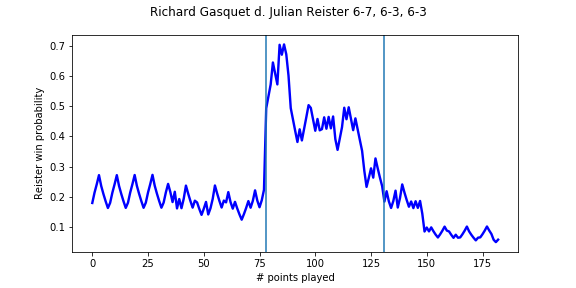
\includegraphics[scale=.7]{gasquet_reister_9_6_all_features}

One drawback of logistic regression is that it cannot distinguish between situations whose score differentials are equivalent. A player serving at (1,1),(5,4),(3,0) will have approximately the same win probability as one serving at (1,1),(1,0),(3,0). However, in the first situation, the player serving wins the match if he wins any of the next three points. From the second scenario, the player serving only holds an early break advantage, from which the returner has many more chances to come back. Assuming each player serves at $f_i=f_j=.64$, our win-probability equation suggests a substantial difference between these two scenarios:

\begin{center}
$P_m(1,1,5,4,3,0) = .994$

$P_m(1,1,1,0,3,0) = .800$
\end{center}

Although the first situation is clearly favorable, logistic regression will compute approximately the same probability in both scenarios $\footnote{after fitting coefficients for the equation $P(win) = logit(s_i,s_j,g_i,g_j,{x}_i,{x}_j)= \frac{e^{(c_1s_i+c_2s_j+c_3g_i+c_4g_j+c_5x_i+c_6x_j}}{1+e^{(c_1s_i+c_2s_j+c_3g_i+c_4g_j+c_5x_i+c_6x_j}}$, coefficients $ c_1 \approx c_2, c_3 \approx c_4,c_5 \approx c_6$ by symmetry and therefore $logit(1,0,5,4,3,0) \approx logit(1,0,1,0dddd,3,0) $}$

%$\footnote{after fitting coefficients for the equation $P(win) = logit(s_i,s_j,g_i,g_j,{x}_i,{x}_j) = \frac{e^{(c_1s_i+c_2s_j+c_3g_i+c_4g_j+c_5x_i+c_6x_j}}{55}$, coefficients $ c_1 \approx c_2, c_3 \approx c_4,c_5 \approx c_6$ by symmetry and therefore}$

Another issue is that logistic regression can fail to detect when a higher-ranked player is about to lose in a close match. Below,

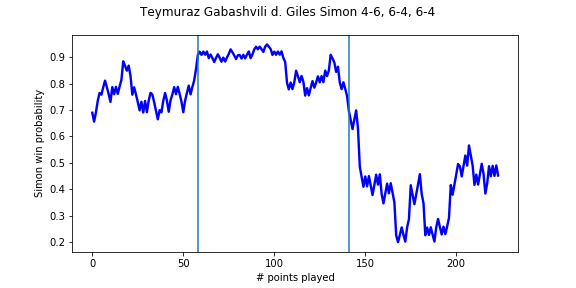
\includegraphics[scale=.7]{simon_gabashvili_9_6_all_features}


\section{Random Forests}
Brian Burke's win-probability models are among the most well-known in sports. They calculate a team's win probability at any point in the match based on historical data. Nettleton and Lock improved upon this method of binning players together with a random forest approach.

\section{Hierarchical Markov Model}
With serving percentages already calculated from historical data, our hierarchical Markov model is well-equipped to produce in-match win probability estimates. Using the analytical equation with players' serving abilities $f_{ij},f_{ji}$, we compute $P_m(s_i,s_j,g_i,g_j,x_i,x_j)$ from every scoreline $(s_i,s_j,g_i,g_j,x_i,x_j)$ in a match. To assess this model's performance, we repeat this on every match in our dataset, testing all estimates of $f_{ij},f_{ji}$ (James-Stein normalized, player-adjusted, elo-induced, surface-specific)

\subsection{Beta Experiments}
The above approaches only take into account the current score when computing win probability. However, in many cases, there is much more information that may be collected from $P_k$. Consider the following in-match substring, 

$P=``SSSS;RSSSRRSS;SSSS;SRRSRSRSSS;SSSS;RRRSSSRSRSSS;"$

The above sequence demonstrates a current scoreline of three games all. However, $p_i$ has won 12/12 service points, while $p_j$ has won 18/30 service points. If both players continue serving at similar rates, $p_i$ is much more likely to break serve and win the match. Since original forecasts are $f_{ij},f_{ji}$ are based on historical serving percentages, it makes sense that in-match serving percentages may help us better determine each player's serving ability on a given day. To do this, we can update $f_{ij},f_{ji}$ at time $t$ of the match to factor in each player's serving performance thus far in the match.

"" attempted this method with beta experiments. The beta distribution is a generalization of the uniform distribution. We often use the beta distribution to represent prior and posterior estimates to some probability parameter $b_{prior}$.

To update our matches with in-match serving statistics, we set $f_{ij}$ as a prior and update with the number of points won and played on $p_i's$ serve, $(s_{won},s_{pt})$. Through beta-binomial conjugacy, we then obtain an update of the form 

$b_{posterior} = \frac{\alpha * f_{ij}+ s_{won}}{\alpha * f_{ij} + s_{pt}}$

where $\alpha$ is a hyper parameter that determines the strength of our prior. Regardless of alpha, the match's influence on our posterior serve estimates will always grow as more points have been played.

\subsection{Elo-adjusted Serve Probabilities}
In "", Klaassen and Magnus suggest a method to infer serving probabilities from a pre-match win forecast $\pi_{ij}$. By imposing a constraint $f_{ij}+f{ji}=1.29$, we can then create a one-to-one function 
$S: S(\pi_{ij}) \rightarrow (f_i,f_j)$, which generates serving probabilities $f_i,f_j$ for both players. Since elo outperformed Klaassen and Magnus' combined player outcome model in pre-match prediction, it makes sense test a version of the hierarchical Markov Model that uses an elo forecast as its starting point.


\section{Results}
 
\end{document}